\documentclass{article}

\title{Optimal Trading\\BT Backtesting Engine}
\author{Jeffrey Wong}
\date{\today}

\usepackage{Sweave}
\begin{document}

\maketitle


\section{Summary}

This R package represents a backtesting engine for Belvedere Trading.  The 
objective is to take a dataset of the market for $n$ different assets over
a period of $T$ days (or any time interval), and use historic prices to determine
what the optimal trading strategy would have been over the past $T$ periods.  
Furthermore, we would like to use data mining techniques to extract any patterns 
from the optimal strategy.  Note: backtesting does not necessarily provide any 
predictive power; it is for us to benchmark our own trading strategies with what 
was best.

\section{Optimization}

In determining the optimal strategy, there are two things we may want to
consider.  In one, we consider pure profit maximization - here, OptimalTrading
will identify the best times to buy and sell the assets.  This is not necessarily
the trivial rule of \textit{buy low, sell high}, as we want to make sure that
funds are not tied up when a good opportunity to buy/sell an asset comes up.
In two, we consider a utility function of profits and risks.  Here, we optimize
to have maximal profits, but also take penalties from any risks we are exposed to.

\subsection{Profit Maximization}

We formulate this problem as a linear program:

$$\min {\mathrm{prices}^T \mathrm{quantity}}$$

subject to:

\begin{itemize}
  \item The amount of liquid funds available at any given time must be greater
    than or equal to 0
  \item The trader cannot short sell an asset
\end{itemize}

Let \textbf{cost} be a vector representing how much money was spent on each
transaction.  This vector is equal to $-\mathrm{prices} \cdot \mathrm{quantity}$.  The running
sum of this vector is equal to the total amount of money spent as of time $t$.  

Likewise, the other constraint can be formulated by considering the running
sum of the quantity vector.  However, this vector contains a mixture of assets,
so we will want to reshape this into a matrix and apply the running sum over each
column.

\subsection{Utility Maximization}

We formulate this problem as a quadratic program:

$$\min {\mathrm{prices}^T \mathrm{quantity} + \frac{1}{2} \mathrm{quantity}^T Q \mathrm{quantity}}$$

subject to:

\begin{itemize}
  \item The amount of liquid funds available at any given time must be greater
    than or equal to 0
  \item The trader cannot short sell an asset
  \item The amount of risk for any particular asset the trader is exposed to 
    should never exceed \textit{riskTol}
\end{itemize}

The utility function is quadratic in the decision variables so to prevent 
buying large quantities of one particular asset.  Q is a diagonal matrix 
containing the risks associated with each transaction.  If Q is positive
definite, then the solution exists and is unique.  If Q is only semi-positive
definite then a solution exists but is not necessarily unique.  If the risks
vector is positive, then Q will be positive definite.  

The risk constraint can be formulated like the previous two, where we compute a
running sum per asset and enforce that this is less than or equal to riskTol.

\section{Application}

Here we will demonstrate the use of OptimalTrading.

First we initialize some parameters and then choose the assets to download 
market data on.

\begin{Schunk}
\begin{Sinput}
> ndays = 10
> initFunds = 10^7
> Symbols = c("GOOG", "AAPL", "NFLX", "AMZN", "V", "BA", "JPM", 
+     "MSFT", "SPY", "RHT", "BBBY", "CSCO", "BAC")
> market = getHistoricData(Symbols, ndays = ndays, return.type = "df", 
+     mergeAll = T)
> head(market)
\end{Sinput}
\begin{Soutput}
         Date   Open   High    Low  Close   Volume Adj.Close
8  2011-06-14 508.15 514.08 506.99 508.37  2341500    508.37
81 2011-06-14 330.00 333.25 329.31 332.44 11938400    332.44
82 2011-06-14 259.80 261.60 255.94 261.13  3045600    261.13
83 2011-06-14 188.99 190.72 187.07 189.96  3960300    189.96
84 2011-06-14  75.11  76.27  74.83  75.93  7508400     75.93
85 2011-06-14  73.34  75.02  73.19  74.64  4775700     74.64
\end{Soutput}
\end{Schunk}

where the function getHistoricData comes from the package \textit{RFinance}.

Now we will extract the prices vector from the market data, and pass it to 
OptimalTrades.  The largest value of profits is returned, as well as the decisions
that we need to make to obtain that.

\begin{Schunk}
\begin{Sinput}
> opt <- OptimalTrades(market$Close, initFunds = initFunds, numAssets = length(Symbols))
> opt$profits
\end{Sinput}
\begin{Soutput}
[1] 1427627
\end{Soutput}
\begin{Sinput}
> opt$decisions
\end{Sinput}
\begin{Soutput}
  [1]  0.000000e+00  0.000000e+00  0.000000e+00  0.000000e+00  0.000000e+00
  [6]  0.000000e+00  0.000000e+00  0.000000e+00  0.000000e+00  0.000000e+00
 [11]  0.000000e+00  0.000000e+00  0.000000e+00  0.000000e+00  0.000000e+00
 [16]  0.000000e+00  0.000000e+00  0.000000e+00  0.000000e+00  0.000000e+00
 [21]  4.212300e+05  0.000000e+00  0.000000e+00  0.000000e+00  0.000000e+00
 [26]  0.000000e+00  0.000000e+00  0.000000e+00  0.000000e+00  1.251039e-11
 [31]  0.000000e+00  0.000000e+00  0.000000e+00 -2.871917e-10  0.000000e+00
 [36]  0.000000e+00  0.000000e+00  0.000000e+00  0.000000e+00  0.000000e+00
 [41]  0.000000e+00  0.000000e+00  0.000000e+00  0.000000e+00  0.000000e+00
 [46] -1.138520e-10 -4.212300e+05  0.000000e+00  2.480349e+05  0.000000e+00
 [51]  0.000000e+00  0.000000e+00  0.000000e+00  0.000000e+00  0.000000e+00
 [56]  0.000000e+00  0.000000e+00  0.000000e+00  0.000000e+00  0.000000e+00
 [61]  0.000000e+00  0.000000e+00  0.000000e+00  0.000000e+00  0.000000e+00
 [66]  0.000000e+00  0.000000e+00  0.000000e+00  0.000000e+00  0.000000e+00
 [71]  0.000000e+00  0.000000e+00  0.000000e+00  0.000000e+00 -2.480349e+05
 [76]  2.007312e+05  0.000000e+00  0.000000e+00  0.000000e+00  0.000000e+00
 [81]  4.364786e-12 -1.172912e-11  0.000000e+00  0.000000e+00  0.000000e+00
 [86]  0.000000e+00  0.000000e+00  0.000000e+00  0.000000e+00  0.000000e+00
 [91]  0.000000e+00  0.000000e+00  0.000000e+00 -4.364786e-12  1.172912e-11
 [96]  0.000000e+00  0.000000e+00  0.000000e+00  0.000000e+00  0.000000e+00
[101]  0.000000e+00 -2.007312e+05  0.000000e+00  0.000000e+00
\end{Soutput}
\end{Schunk}

The decisions vector can be long and hard to read.  We need a way to visualize this.

\begin{Schunk}
\begin{Sinput}
> (OptimalTrades.Decisions.plot(opt$decisions, length(Symbols), 
+     Symbols))
\end{Sinput}
\begin{Soutput}
$decisions.matrix
  GOOG AAPL NFLX AMZN V BA JPM MSFT SPY RHT BBBY CSCO BAC
1    0    0    0    0 0  0   0    0   0   0    0    0   0
2    0    0    0    0 0  0   0    2   0   0    0    0   0
3    0    0    0    0 0  0   0    0   0   0    0    0   0
4    0    0    0    0 0  0   0   -2   0   2    0    0   0
5    0    0    0    0 0  0   0    0   0   0    0    0   0
6    0    0    0    0 0  0   0    0   0  -2    2    0   0
7    0    0    0    0 0  0   0    0   0   0    0    0   0
8    0    0    0    0 0  0   0    0   0   0   -2    0   0

$decisions.clean
  [1]       0.0       0.0       0.0       0.0       0.0       0.0       0.0
  [8]       0.0       0.0       0.0       0.0       0.0       0.0       0.0
 [15]       0.0       0.0       0.0       0.0       0.0       0.0  421230.0
 [22]       0.0       0.0       0.0       0.0       0.0       0.0       0.0
 [29]       0.0       0.0       0.0       0.0       0.0       0.0       0.0
 [36]       0.0       0.0       0.0       0.0       0.0       0.0       0.0
 [43]       0.0       0.0       0.0       0.0 -421230.0       0.0  248034.9
 [50]       0.0       0.0       0.0       0.0       0.0       0.0       0.0
 [57]       0.0       0.0       0.0       0.0       0.0       0.0       0.0
 [64]       0.0       0.0       0.0       0.0       0.0       0.0       0.0
 [71]       0.0       0.0       0.0       0.0 -248034.9  200731.2       0.0
 [78]       0.0       0.0       0.0       0.0       0.0       0.0       0.0
 [85]       0.0       0.0       0.0       0.0       0.0       0.0       0.0
 [92]       0.0       0.0       0.0       0.0       0.0       0.0       0.0
 [99]       0.0       0.0       0.0 -200731.2       0.0       0.0
\end{Soutput}
\end{Schunk}
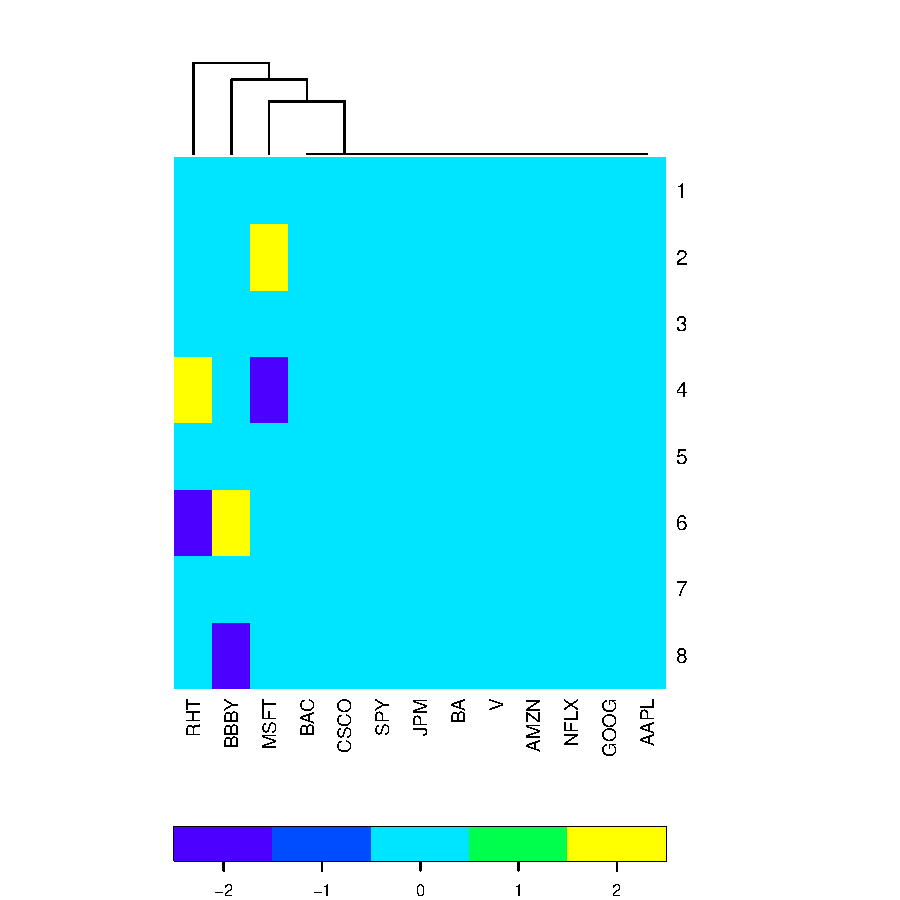
\includegraphics{OptimalTrading-004}

This is a heatmap of the decisions vector, which is transformed into a decisions 
\textit{matrix} first.  The values in the decisions vector are binned into 5
categories, 2 if buying a large quantity, 1 if buying a small quantity, 0 if no 
trade was made, -1 if selling a small quantity, -2 if selling a large quantity.
The image of the matrix is then plotted.

But of course, we are risk averse people.  We will generate some random data to
represent the risks for each transaction.

\begin{Schunk}
\begin{Sinput}
> set.seed(100)
> n = length(market$Close)
> risks = abs(rnorm(n))
> riskTol = initFunds
\end{Sinput}
\end{Schunk}

By specifying a risks vector and riskTol scalar, OptimalTrades will switch
the objective function and use quadratic programming.

\begin{Schunk}
\begin{Sinput}
> opt <- OptimalTrades(market$Close, risks, riskTol, initFunds, 
+     length(Symbols))
\end{Sinput}
\begin{Soutput}
[1] "D matrix is positive definite.  A unique solution should be found"
\end{Soutput}
\begin{Sinput}
> opt$profits
\end{Sinput}
\begin{Soutput}
[1] 903.6935
\end{Soutput}
\end{Schunk}

Visualizing the decisions, we will see that the trades are much more diversified.

\begin{Schunk}
\begin{Sinput}
> (OptimalTrades.Decisions.plot(opt$decisions, length(Symbols), 
+     Symbols))
\end{Sinput}
\begin{Soutput}
$decisions.matrix
  GOOG AAPL NFLX AMZN  V BA JPM MSFT SPY RHT BBBY CSCO BAC
1    0    0    0    2  0  0   0    1   0   0    0    2   0
2    0    0    0    2  1  1   0    2   2   2    2    1   1
3    0    0    2    2 -1  1   1    2   2   2    2    1   1
4    2    2    2    2  1 -1  -1   -1   1   2    2    1  -1
5    2    2    2    2  1 -1   1   -1   2  -2    2    1   1
6   -2   -2   -2   -2 -2  0  -1   -1  -1  -1   -2   -1  -1
7   -1   -1    2   -2  1  0  -1   -2  -2  -2   -1   -2  -1
8    0   -2   -2   -2 -1  0   0   -1  -1  -2   -2   -1  -1

$decisions.clean
  [1]   0.000000000   0.000000000   0.000000000   1.543782118   0.000000000
  [6]   0.000000000   0.000000000   0.049341378   0.000000000   0.000000000
 [11]   0.000000000   1.181541025   0.000000000   0.000000000   0.000000000
 [16]   0.000000000  13.755803295   0.066448514   0.278947241   0.000000000
 [21]   1.176142004   1.289385401   1.248310732   1.329430700   0.434382726
 [26]   0.371092419   0.000000000   0.000000000   2.150567596  31.079517059
 [31]  -0.066448514   0.054004360   0.917095940   2.295602164   1.021962275
 [36]   3.593461793   5.894710346   0.344462505   0.058856341   1.223865303
 [41]  13.603774919   4.361288663   2.791012236   0.709629149  -0.105486904
 [46]  -0.237103293  -0.013052959   0.724125094  12.266343720   1.037011532
 [51]   0.500494637  -0.009947278   9.098470707   3.332097800   2.711257699
 [56]   3.680912323   0.587639265  -0.227464698   0.004701870  -0.255997487
 [61]   1.164784452  -3.093818225   3.558317038   0.020818389   0.482967604
 [66]  -9.526459244  -5.732745640  -9.223113958 -41.492049382  -1.275762809
 [71]   0.000000000  -0.397898301  -0.434218498  -0.876440604  -0.976186797
 [76]  -9.554105970  -0.290794972  -0.618372999  -0.795876765  -0.466378952
 [81]   3.436537333  -6.020459087   0.157583503   0.000000000  -0.286796216
 [86]  -2.499882156  -3.072689985  -2.426086269  -0.070526804  -1.602074848
 [91]  -0.228485415   0.000000000 -10.736748127  -3.436537333  -5.338518564
 [96]  -0.179089108   0.000000000   0.000000000  -0.317934446  -0.251126633
[101] -10.612024955  -2.194836843  -0.588829462  -0.056110672
\end{Soutput}
\end{Schunk}
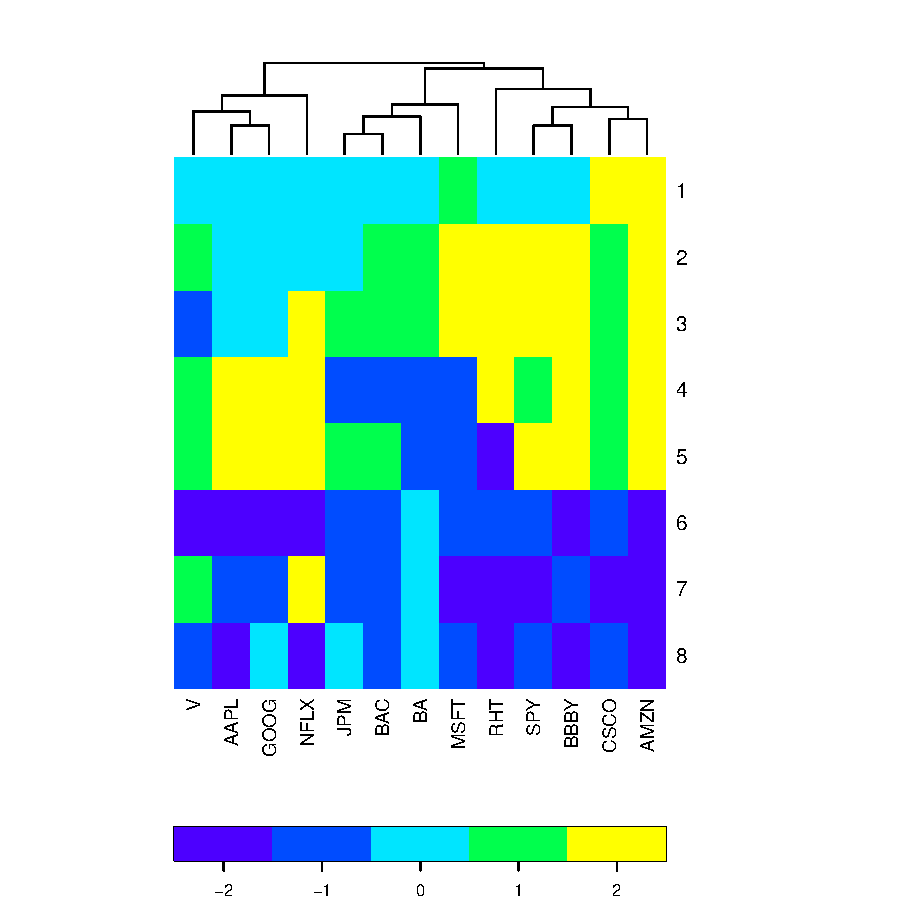
\includegraphics{OptimalTrading-007}

From this strategy, we would like to see if there are any patterns to what
should be bought together and what should be sold together.  We can run
association rules analysis using the apriori algorithm from the \textit{arules}
package.

\begin{Schunk}
\begin{Sinput}
> rules = OptimalTrades.Decisions.FindAssociations(opt$decisions, 
+     length(Symbols), Symbols, parameter = list(supp = 0.5, conf = 0.9, 
+         target = "rules"))
\end{Sinput}
\begin{Soutput}
parameter specification:
 confidence minval smax arem  aval originalSupport support minlen maxlen
        0.9    0.1    1 none FALSE            TRUE     0.5      1     10
 target   ext
  rules FALSE

algorithmic control:
 filter tree heap memopt load sort verbose
    0.1 TRUE TRUE  FALSE TRUE    2    TRUE

apriori - find association rules with the apriori algorithm
version 4.21 (2004.05.09)        (c) 1996-2004   Christian Borgelt
set item appearances ...[0 item(s)] done [0.00s].
set transactions ...[13 item(s), 8 transaction(s)] done [0.00s].
sorting and recoding items ... [7 item(s)] done [0.00s].
creating transaction tree ... done [0.00s].
checking subsets of size 1 2 3 4 5 done [0.00s].
writing ... [64 rule(s)] done [0.00s].
creating S4 object  ... done [0.00s].

parameter specification:
 confidence minval smax arem  aval originalSupport support minlen maxlen
        0.9    0.1    1 none FALSE            TRUE     0.5      1     10
 target   ext
  rules FALSE

algorithmic control:
 filter tree heap memopt load sort verbose
    0.1 TRUE TRUE  FALSE TRUE    2    TRUE

apriori - find association rules with the apriori algorithm
version 4.21 (2004.05.09)        (c) 1996-2004   Christian Borgelt
set item appearances ...[0 item(s)] done [0.00s].
set transactions ...[13 item(s), 8 transaction(s)] done [0.00s].
sorting and recoding items ... [6 item(s)] done [0.00s].
creating transaction tree ... done [0.00s].
checking subsets of size 1 2 3 done [0.00s].
writing ... [9 rule(s)] done [0.00s].
creating S4 object  ... done [0.00s].
\end{Soutput}
\begin{Sinput}
> inspect(rules$buy.rules)
\end{Sinput}
\begin{Soutput}
   lhs       rhs    support confidence lift
1  {SPY}  => {BBBY}   0.500          1  2.0
2  {BBBY} => {SPY}    0.500          1  2.0
3  {SPY}  => {NFLX}   0.500          1  1.6
4  {SPY}  => {CSCO}   0.500          1  1.6
5  {SPY}  => {AMZN}   0.500          1  1.6
6  {BBBY} => {NFLX}   0.500          1  1.6
7  {BBBY} => {CSCO}   0.500          1  1.6
8  {BBBY} => {AMZN}   0.500          1  1.6
9  {CSCO} => {AMZN}   0.625          1  1.6
10 {AMZN} => {CSCO}   0.625          1  1.6
11 {V,                                     
    CSCO} => {AMZN}   0.500          1  1.6
12 {AMZN,                                  
    V}    => {CSCO}   0.500          1  1.6
13 {SPY,                                   
    BBBY} => {NFLX}   0.500          1  1.6
14 {NFLX,                                  
    SPY}  => {BBBY}   0.500          1  2.0
15 {NFLX,                                  
    BBBY} => {SPY}    0.500          1  2.0
16 {SPY,                                   
    BBBY} => {CSCO}   0.500          1  1.6
17 {SPY,                                   
    CSCO} => {BBBY}   0.500          1  2.0
18 {BBBY,                                  
    CSCO} => {SPY}    0.500          1  2.0
19 {SPY,                                   
    BBBY} => {AMZN}   0.500          1  1.6
20 {AMZN,                                  
    SPY}  => {BBBY}   0.500          1  2.0
21 {AMZN,                                  
    BBBY} => {SPY}    0.500          1  2.0
22 {NFLX,                                  
    SPY}  => {CSCO}   0.500          1  1.6
23 {SPY,                                   
    CSCO} => {NFLX}   0.500          1  1.6
24 {NFLX,                                  
    CSCO} => {SPY}    0.500          1  2.0
25 {NFLX,                                  
    SPY}  => {AMZN}   0.500          1  1.6
26 {AMZN,                                  
    SPY}  => {NFLX}   0.500          1  1.6
27 {NFLX,                                  
    AMZN} => {SPY}    0.500          1  2.0
28 {SPY,                                   
    CSCO} => {AMZN}   0.500          1  1.6
29 {AMZN,                                  
    SPY}  => {CSCO}   0.500          1  1.6
30 {NFLX,                                  
    BBBY} => {CSCO}   0.500          1  1.6
31 {BBBY,                                  
    CSCO} => {NFLX}   0.500          1  1.6
32 {NFLX,                                  
    CSCO} => {BBBY}   0.500          1  2.0
33 {NFLX,                                  
    BBBY} => {AMZN}   0.500          1  1.6
34 {AMZN,                                  
    BBBY} => {NFLX}   0.500          1  1.6
35 {NFLX,                                  
    AMZN} => {BBBY}   0.500          1  2.0
36 {BBBY,                                  
    CSCO} => {AMZN}   0.500          1  1.6
37 {AMZN,                                  
    BBBY} => {CSCO}   0.500          1  1.6
38 {NFLX,                                  
    CSCO} => {AMZN}   0.500          1  1.6
39 {NFLX,                                  
    AMZN} => {CSCO}   0.500          1  1.6
40 {NFLX,                                  
    SPY,                                   
    BBBY} => {CSCO}   0.500          1  1.6
41 {SPY,                                   
    BBBY,                                  
    CSCO} => {NFLX}   0.500          1  1.6
42 {NFLX,                                  
    SPY,                                   
    CSCO} => {BBBY}   0.500          1  2.0
43 {NFLX,                                  
    BBBY,                                  
    CSCO} => {SPY}    0.500          1  2.0
44 {NFLX,                                  
    SPY,                                   
    BBBY} => {AMZN}   0.500          1  1.6
45 {AMZN,                                  
    SPY,                                   
    BBBY} => {NFLX}   0.500          1  1.6
46 {NFLX,                                  
    AMZN,                                  
    SPY}  => {BBBY}   0.500          1  2.0
47 {NFLX,                                  
    AMZN,                                  
    BBBY} => {SPY}    0.500          1  2.0
48 {SPY,                                   
    BBBY,                                  
    CSCO} => {AMZN}   0.500          1  1.6
49 {AMZN,                                  
    SPY,                                   
    BBBY} => {CSCO}   0.500          1  1.6
50 {AMZN,                                  
    SPY,                                   
    CSCO} => {BBBY}   0.500          1  2.0
51 {AMZN,                                  
    BBBY,                                  
    CSCO} => {SPY}    0.500          1  2.0
52 {NFLX,                                  
    SPY,                                   
    CSCO} => {AMZN}   0.500          1  1.6
53 {NFLX,                                  
    AMZN,                                  
    SPY}  => {CSCO}   0.500          1  1.6
54 {AMZN,                                  
    SPY,                                   
    CSCO} => {NFLX}   0.500          1  1.6
55 {NFLX,                                  
    AMZN,                                  
    CSCO} => {SPY}    0.500          1  2.0
56 {NFLX,                                  
    BBBY,                                  
    CSCO} => {AMZN}   0.500          1  1.6
57 {NFLX,                                  
    AMZN,                                  
    BBBY} => {CSCO}   0.500          1  1.6
58 {AMZN,                                  
    BBBY,                                  
    CSCO} => {NFLX}   0.500          1  1.6
59 {NFLX,                                  
    AMZN,                                  
    CSCO} => {BBBY}   0.500          1  2.0
60 {NFLX,                                  
    SPY,                                   
    BBBY,                                  
    CSCO} => {AMZN}   0.500          1  1.6
61 {NFLX,                                  
    AMZN,                                  
    SPY,                                   
    BBBY} => {CSCO}   0.500          1  1.6
62 {AMZN,                                  
    SPY,                                   
    BBBY,                                  
    CSCO} => {NFLX}   0.500          1  1.6
63 {NFLX,                                  
    AMZN,                                  
    SPY,                                   
    CSCO} => {BBBY}   0.500          1  2.0
64 {NFLX,                                  
    AMZN,                                  
    BBBY,                                  
    CSCO} => {SPY}    0.500          1  2.0
\end{Soutput}
\begin{Sinput}
> inspect(rules$sell.rules)
\end{Sinput}
\begin{Soutput}
  lhs       rhs    support confidence lift
1 {AAPL} => {GOOG}     0.5          1  1.6
2 {RHT}  => {MSFT}     0.5          1  1.6
3 {JPM}  => {BAC}      0.5          1  2.0
4 {BAC}  => {JPM}      0.5          1  2.0
5 {JPM}  => {MSFT}     0.5          1  1.6
6 {BAC}  => {MSFT}     0.5          1  1.6
7 {JPM,                                   
   BAC}  => {MSFT}     0.5          1  1.6
8 {JPM,                                   
   MSFT} => {BAC}      0.5          1  2.0
9 {MSFT,                                  
   BAC}  => {JPM}      0.5          1  2.0
\end{Soutput}
\end{Schunk}

\end{document}
